\documentclass[11pt,a4paper,twoside,french,svgnames]{report}
\usepackage[utf8]{inputenc} % force the use of utf8
\usepackage[T1]{fontenc} % font encoding, allows accents (T1 font encoding is an 8-bit encoding)
\usepackage[top=2.5cm,bottom=2.5cm,outer=2.5cm,inner=2.5cm]{geometry} % http://tex.stackexchange.com/questions/62311/a4paper-where-should-i-declare-it-in-document-class-or-geometry // another option: papersize={21cm,29.7cm}
\usepackage[french]{babel} % translate everything in the desired language: table of contents, etc. 'english' can be replaced with 'francais'
\usepackage[toc,page,header]{appendix} % cool appendices
\usepackage{graphicx} % images management
\usepackage{wrapfig} % floating images
\usepackage[format=plain,labelfont=bf,font=small,justification=centering,margin=10pt]{caption} % allow multiline captions in figures,
\usepackage{float} % allow \begin{figure}[H] and \begin{table}[H] (to really force positionning, unlike h!)
\usepackage{array} % allow arrays
\usepackage[super]{nth} % allow to write \nth(1) to write 1st, etc
\usepackage{fancyhdr} % headers/footers management (overrides empty, plain and headings)
\usepackage{upquote} % without this, lslisting replace vertical singles quotes with curved ones
\usepackage{listings} % code insertion (MUST BE WRITTEN AFTER BABEL)
\usepackage[
            backend=biber,
            style=numeric,
            sorting=none, % nty = name title year
            url=true, % always show url when provided
            ]{biblatex}
%\usepackage{pdfpages} % include PDF documents
\usepackage{enumitem} % for /setlist
\usepackage{color,soul} % add some colors and hightlight
\usepackage{xcolor} % more colors
\usepackage{afterpage} % allow to execute command after the current page ends
\usepackage[hidelinks,
            colorlinks  = false, % no borders, colors enabled
            anchorcolor = blue,
            linkcolor   = black, % links in table of contents
            urlcolor    = blue,
            citecolor   = blue,
            breaklinks  = true]{hyperref}
\newcommand{\MYhref}[3][blue]{\href{#2}{\color{#1}{#3}}}%

% List settings
\setlist{itemsep=.5em}
\setlist[itemize,2]{label={$\bullet$}} % use bullets for nested itemize in level 2

% REQUIRE
% \usepackage{color}
% \usepackage{listings} % (MUST BE WRITTEN AFTER BABEL)

% General colors
\definecolor{comment}{rgb}{0.12, 0.38, 0.18 } % adjusted, in Eclipse: {0.25, 0.42, 0.30 } = #3F6A4D
\definecolor{keyword}{rgb}{0.2, 0.2, 0.8}
\definecolor{string}{rgb}{0.06, 0.10, 0.98} % #101AF9

% Language-specific colors
% JavaScript
\definecolor{darkgray}{rgb}{.4,.4,.4}
%\definecolor{purple}{rgb}{0.65, 0.12, 0.82}

% hack to force UTF-8 compatibility (for french only)
\lstset{
       extendedchars=true,
       literate={à}{{\`a}}1 {â}{{\^a}}1 %                         lettre a
                {À}{{\`A}}1 {Â}{{\^A}}1 %                         lettre A
                {ç}{{\c{c}}}1 %                                   lettre c
                {Ç}{{\c{C}}}1 %                                   lettre C
                {é}{{\'e}}1 {è}{{\`e}}1 {ê}{{\^e}}1 {ë}{{\"e}}1 % lettre e
                {É}{{\'E}}1 {È}{{\`E}}1 {Ê}{{\^E}}1 {Ë}{{\"E}}1 % lettre E
                {î}{{\^i}}1 {ï}{{\"i}}1 %                         lettre i
                {Î}{{\^I}}1 {Ï}{{\"I}}1 %                         lettre I
                {ô}{{\^o}}1 %                                     lettre o
                {Ô}{{\^O}}1 %                                     lettre O
                {œ}{{\oe}}1 %                                     lettre oe
                {Œ}{{\OE}}1 %                                     lettre OE
                {ù}{{\`u}}1 {û}{{\^u}}1 {ü}{{\"u}}1 %             lettre u
                {Ù}{{\`U}}1 {Û}{{\^U}}1 {Ü}{{\"U}}1 %             lettre U
}

% General rules
\lstset{
  rulecolor=\color{black!50},
  backgroundcolor = \color{blue!10},
  numbers=none, %left % display line numbers
  showspaces=false,
  showtabs=false,
  breaklines=true,
  showstringspaces=false,
  breakatwhitespace=false,
  commentstyle=\color{comment},
  keywordstyle=\color{keyword},
  stringstyle=\color{string},
  basicstyle=\ttfamily,
  extendedchars=true,
  emph=[2]{In},
  emphstyle=[2]\color{black!70},
  morecomment=[l][\color{blue}]{Out},
  frame=single,
  frameround=tttt,
  framerule=0.3pt,
  framesep=4pt,
  belowcaptionskip=2.1pt
}

% % Define "Javascript" because lstlistings doesn't know it
% Taken from https://gist.github.com/Geruhn/3d21f60a869457373d84
\lstdefinelanguage{javascript}{
  keywords={break, case, catch, continue, debugger, default, delete, do, else, false, finally, for, function, if, in, instanceof, new, null, return, switch, this, throw, true, try, typeof, var, void, while, with},
  morecomment=[l]{//},
  morecomment=[s]{/*}{*/},
  morestring=[b]',
  morestring=[b]",
  ndkeywords={class, export, boolean, throw, implements, import, this},
  %keywordstyle=\color{blue}\bfseries,
  ndkeywordstyle=\color{darkgray}\bfseries,
  identifierstyle=\color{black},
  %commentstyle=\color{purple}\ttfamily,
  %stringstyle=\color{red}\ttfamily,
  sensitive=true
}

% Usage: \javascript
\newcommand{\javascript}{\lstset{
  language=javascript,
  title={{\setlength{\fboxsep}{1pt}\fcolorbox{orange}{yellow!20}{\sffamily\scriptsize
              \textcolor{gray!10}{\_}JavaScript\textcolor{gray!10}{\_}}}}
  }
}

% Usage: \code{My title}
\newcommand{\code}[1]{\lstset{
  language=,
  title={{\setlength{\fboxsep}{1pt}\fcolorbox{orange}{yellow!20}{\sffamily\scriptsize
              \textcolor{gray!10}{\_}{#1}\textcolor{gray!10}{\_}}}}
  }
}

% Usage: \sql
\newcommand{\sql}{\lstset{
  language=SQL,
  title={{\setlength{\fboxsep}{1pt}\fcolorbox{orange}{yellow!20}{\sffamily\scriptsize
              \textcolor{gray!10}{\_}SQL\textcolor{gray!10}{\_}}}}
  }
}

% Usage: \fakeshell
\newcommand{\fakeshell}{\lstset{
  language=bash
  }
}

\newcommand{\java}{\lstset{
  language=java,
  title={{\setlength{\fboxsep}{1pt}\fcolorbox{orange}{yellow!20}{\sffamily\scriptsize
              \textcolor{gray!10}{\_}Java\textcolor{gray!10}{\_}}}}
  }
}

\newcommand{\perl}{\lstset{
  language=perl
  }
}

\newcommand{\xml}{\lstset{
  language=xml
  }
}

% REQUIRES
% Nothing

% Redefine chapter titles: only display the title and remove useless blank space
% Original "/usr/share/texlive/texmf-dist/tex/latex/base/report.cls" edited
\makeatletter
  \def\@makechapterhead#1{% chapter{}
  \vspace*{0\p@}% 50 before
  {\parindent \z@ \raggedright \normalfont
    %\ifnum \c@secnumdepth >\m@ne
    %    \huge\bfseries \@chapapp\space \thechapter
    %    \par\nobreak
    %    \vskip 20\p@
    %\fi
    \interlinepenalty\@M
    \Huge \bfseries \thechapter\quad #1   
    \vskip 40\p@
  }}
  \def\@makeschapterhead#1{% chapter*{}
  \vspace*{0\p@}% 50 before
  {\parindent \z@ \raggedright
    \normalfont
    \interlinepenalty\@M
    \Huge \bfseries  #1\par\nobreak
    \vskip 40\p@
  }}
\makeatother
% REQUIRES
% \usepackage{fancyhdr} % headers/footers management (overrides empty, plain and headings)

% THE ORDER IS REALLY IMPORTANT, OTHERWISE IT WILL BREAK THINGS

% 1.
% Redefines the existing 'plain' style, (because 'chapter' and \tableofcontents ignores the page style currently in effect for their first page)
\fancypagestyle{plain}{
    % Took from: http://anorien.csc.warwick.ac.uk/mirrors/CTAN/macros/latex/contrib/fancyhdr/fancyhdr.pdf
    \fancyhead[LO,RE]{\slshape \leftmark}
    \fancyhead[LE,RO]{\slshape \rightmark}

    % Footers
    \renewcommand{\footrulewidth}{0.4pt}
    \fancyfoot[C]{Rapport de TD -- Steve \textsc{Lagache} \& Romain \textsc{Pellerin}}
    \fancyfoot[LE,RO]{\ifdefined\thepage \thepage \fi} % to be used with \pagenumbering{gobble} % no numerotation
    % \fancyfoot[LE,RO]{\ifnum\thepage>0 \thepage \fi} % to be used with %\addtocounter{page}{-4} % numerotation begins at 1 + (-4)
}

% 2.
\pagestyle{plain}

% 3.
% http://tex.stackexchange.com/questions/111223/markboth-is-not-working-when-using-chapter-and-section
% Took from : http://ftp.snt.utwente.nl/pub/software/tex/macros/latex/contrib/fancyhdr/fancyhdr.pdf
\renewcommand{\chaptermark}[1]{\markboth{}{\MakeUppercase{\thechapter.\ #1}}}
\renewcommand{\sectionmark}[1]{}

% NORMALLY
% \renewcommand{\chaptermark}[1]{\markboth{\MakeUppercase{\thechapter.\ #1}}{}}
% \renewcommand{\sectionmark}[1]{\markright{\thesection.\ #1}}
 % To be edited to change the header and footer

\title{Rapport de TD}
\author{Steve LAGACHE et Romain PELLERIN}
\date\today
\setcounter{tocdepth}{2} % ToC depth

\pagenumbering{arabic} % re-enable numering

\begin{document}
\thispagestyle{empty} % only applies to this page
\begin{center}

\includegraphics[height=3cm]{images/logo-utc.png}

\vspace{4cm}

\noindent{\LARGE\MYhref[black]{http://www.utc.fr/}{Université de Technologie de Compiègne}}

\vspace{1cm}

{\large Génie Informatique}

\vspace{3cm}
\noindent\fbox{
\begin{minipage}{.9\textwidth}
\begin{center}
    \vspace{0.3cm}\Large{Rapport de TD}\\
    \vspace{0.3cm}\LARGE{\textbf{LO17}}\vspace{0.3cm}\\
\end{center}
\end{minipage}}

\vspace{3cm}

\begin{tabular}{>{\hfill\arraybackslash}p{5cm}p{5cm}}
%\hline
    \multicolumn{2}{c}{\textbf{Steve \textsc{LAGACHE} \& Romain \textsc{PELLERIN}}}\\\\
%\hline
    \multicolumn{2}{c}{Chargé de TD : Pierre \textsc{Morizet-Mahoudeaux}}\\\\
%\hline
    \multicolumn{2}{c}{Printemps 2016 (P16)}\\
%\hline

\end{tabular}
\vfill

{\footnotesize Dernière mise à jour: \today}
\end{center}


\tableofcontents

\chapter{Introduction}

Ce rapport est une synthèse critique d'un ensemble de trois TD réalisés dans le cadre de l'UV LO17. Le but final de ces trois TD est de développer un logiciel permettant à l'utilisateur de saisir une requête en langage naturel afin d'obtenir des résultats extraits d'une base de données.

\medskip

Cette base de données a été préalablement remplie après avoir analysé un certain nombre de pages d'articles d'un site d'information. Ces pages ont été \textit{parsées} afin d'en obtenir des termes significatifs. À présent, nous avons à disposition dans cette base de données plusieurs tables qui contiennent diverses informations organisées, telles que des dates de parution d'articles, les rubriques, les mots significatifs retenus pour chaque article, etc.

\medskip

Notre travail pour ce projet, encore inachevé, a été séparé en trois étapes distinctes :

\begin{enumerate}
  \item \textbf{TD 3} : transformer une phrase en une suite des lemmes. Il s'agissait tout d'abord de permettre à l'utilisateur de rentrer une phrase. Suite à cela, nous devions retirer de cette phrase des mots faisant partie d'une stop list. Puis, finalement, il nous fallait ``transformer'' chaque mot en un ``lemme'', soit directement à partir d'une liste déjà fournie, soit indirectement en utilisant un algorithme (au choix celui de proximité ou de Levenshtein). Il nous a également fallu prendre en considération les erreurs de saisies éventuelles de l'utilisateur.
  \item \textbf{TD 4} : faire de l'analyse syntaxique à l'aide d'Antlr. À partir de la phrase ``\textit{lémmatisée}'' obtenue suite au TD 3, il nous a fallu écrire une grammaire capable de reconnaître chaque terme afin de construire un arbre syntaxique (donc une requête SQL syntaxiquement correcte). Le TD consistait tout d'abord à prendre en main le logiciel à l'aide d'une grammaire déjà fournie puis ensuite à créer notre propre grammaire en partant d'un exemple.
  \item \textbf{TD 6} : ce dernier TP a été l'occasion de créer une petite application Java permettant d'exécuter une requête SQL sur une base de données PostgreSQL mise à disposition sur les serveurs de l'UTC. Il s'agissait principalement d'être capable de transmettre une requête SQL entrée par l'utilisateur et d'afficher les résultats correctement, en utilisant chaque colonne de chaque ligne des résultats.
\end{enumerate}

On peut aisément distinguer ici les différentes étapes qui, une fois les TD ``assemblés'', permettront d'obtenir des résultats SQL à partir d'une requête donnée en langage naturel.

\medskip

Nous présenterons donc dans ce rapport la réalisation de ces trois TP ainsi que la mise en commun de tout le code afin d'obtenir l'application fonctionnelle décrite plus haut.

\chapter{TD3: Correcteur orthographique}

\section{Ambition}

Le but de ce TD était d'obtenir un analyseur associant à chaque mot d'une phrase donnée en argument, le lemme lui correspondant, ou à défaut une liste des meilleurs lemmes possibles. Les erreurs éventuelles dues à l'utilisateur étaient également à prendre en compte.

\medskip

Par ailleurs, comme dit précédemment, il nous était demandé d'implémenter deux algorithmes : celui par \textbf{proximité} et celui de \textbf{Levenshtein}. À la sortie de ces algorithmes, nous aurions donc une phrase composée uniquement de lemmes, prête à être transformée en requête SQL. Au préalable, avant la transformation en lemmes, il nous fallait retirer les mots présents dans la stop list fournie ainsi que ceux présents dans notre stop list, que nous viendrions compléter au fur et à mesure du projet. Cela n'était pas précisé dans le sujet mais il était néanmoins important de le faire pour la suite du projet.

\section{Fonctionnement et structuration}

\subsection{Récupération des fichiers de stop lists et de lemmes}

Nous avons deux classes pour cela :

\java
\begin{itemize}
    \item \lstinline{Main.java} : entrée du programme (contient la fonction \lstinline{main}). Cette classe lit les paramètres donnés au programme grâce à \lstinline{String[] args}. Les paramètres données en entrée au programme sont les fichiers de stop list et de lemmes.
    \item \lstinline{InputFile.java} : classe permettant d'obtenir une \lstinline{ArrayList<String>} contenant toutes les lignes d'un fichier.
\end{itemize}

Nous instancions donc 4 fois la classe \lstinline{InputFile}: 2 fois pour récupérer la stop list et les lemmes fournis dans le cadre du TD, 2 autres fois supplémentaires pour récupérer nos propres fichiers (une stop liste et un autre ensemble de lemmes). Par conséquent, notre programme accepte 4 arguments.\\
\textbf{Pourquoi créer deux fichiers supplémentaires ?} Nous avions besoin de supprimer certains mots comme ``\textbf{d'}'' ou ``\textbf{l'}'' pour plus tard obtenir une phrase prête à être interprétée par la grammaire. De même, en vue d'obtenir une requête SQL, il nous fallait avoir nos propres lemmes, tels que :

\begin{itemize}
  \item veux: vouloir
  \item afficher:    vouloir
  \item lister:      vouloir
\end{itemize}

Il est important de noter que si une association mot-lemme a été définie dans le fichier fourni pour le TD, elle peut être supprimée et remplacée par une autre association mot-lemme définie dans notre fichier, où le mot serait le même. Par exemple, si le mot ``afficher'' avait été associé au lemme ``affiche'' dans le fichier du TD, notre fichier viendrait écraser cette association et au final, le lemme correspondant à ``afficher'' serait ``vouloir'', comme défini dans notre fichier de lemmes. Cela se fait grâce à l'utilisation de \java\lstinline{HashMap<String,String>}, qui offre de bonnes performances en termes de temps d'accès (temps constant) et assure aussi l'unicité des clés.

\subsection{Saisie de la phrase par l'utilisateur}

Nous avons créé une classe qui lit sur \lstinline{System.in} et retourne une \lstinline{String} correspondant à ce que l'utilisateur a entré.

\subsection{Retirer les mots des stop lists}

La phrase entrée par l'utilisateur est mise en minuscules et \textit{tokenizée} grâce à \lstinline{string.split("\\s+")}. Cela nous permet d'obtenir un tableau de \lstinline{String} sur lequel itérer.

\medskip

Nous avons créé une classe \lstinline{Lexicon.java} qui contient nos deux algorithmes (proximité et Levenshtein, voir plus bas) ainsi qu'un \lstinline{HashMap<String,String>}.

\medskip

Les mots de la stop list ont au préalable été mis dans le \lstinline{HashMap<String,String>} (qui est un attribut de la classe \lstinline{Lexicon}), pour lequel la clé vaut le mot de la stop list et la valeur vaut une \lstinline{String} vide. Avec une simple boucle \lstinline{for} sur les tokens, nous remplaçons les mots si présents dans le \lstinline{HashMap} par la valeur associée, c'est-à-dire une \lstinline{String} vide.

\subsection{Trouver le lemme ``parfait''}

Ici, le principe est le même, nous utilisons un objet de la classe \lstinline{Lexicon}. Le \lstinline{HashMap} contient en clés les mots à remplacer et en valeurs les lemmes associés. Une fois de plus, comme pour la stop list, une boucle \lstinline{for} permet de remplacer les mots par leur lemme correspondant, s'il y en a un.

\subsection{Trouver le lemme par préfixe}

Si nous ne trouvons pas de lemme associé à un mot donné, nous lançons l'algorithme de recherche par préfixe (implémenté selon le pseudo-code fourni dans le polycopié). \textbf{Cet algorithme suppose que le mot diffère uniquement par sa terminaison et qu'il n'y a pas de faute de frappe.} Le mot que l'on cherche à remplacer est comparé avec tous les mots présents en tant que clés de notre \lstinline{HashMap}. Si un mot a une très grande proximité avec le mot que l'on cherche à remplacer, on utilisera son lemme associé.

\subsubsection{Seuils}

Nous avons choisi les seuils suivants :

\begin{itemize}
    \item \textbf{SEUIL\_MIN} = 4 : correspondant au nombre minimum de lettres par mot pour les comparer
    \item \textbf{SEUIL\_MAX} = 1 : correspond à la différence entre le nombre de lettres des deux mots à comparer
    \item \textbf{SEUIL\_PROX} = 0.80 : correspond au pourcentage de correspondance minimum entre les deux mots pour que le mot trouvé soit retenu (donc 80\%)
\end{itemize}

Après plusieurs essais, ces seuils nous ont semblé donner de bons résultats. Il faut un minimum de lettres dans chaque mot pour les comparer mais surtout il ne faut pas une trop grande différence entre les nombres de lettres. Cet algorithme est peu fiable car il suppose qu'il n'y a pas de faute de frappe et que seule la fin change légèrement. Nous avons donc mis des seuils stricts pour être vraiment sûrs que le lemme ait de grandes chances d'être le bon. Sinon, nous préférerons nous référer à l'algorithme de Levenshtein.

\medskip

Après avoir lancé l'algorithme avec chaque mot de notre dictionnaire de lemmes, seul le mot ayant la plus grande proximité, supérieure à 80\% sera retenu. En cas d'égalité entre plusieurs mots, le premier est retenu.

\subsection{Trouver le lemme par Levenshtein}

Dans le cas où aucun lemme correspondant n'est trouvé directement dans le lexique ou avec une recherche par préfixe, il faut prendre en compte la possibilité qu'on ne trouve aucune correspondance pour le mot analysé car il comporte des fautes, probablement dues à l'utilisateur lorsqu'il a rentré sa phrase au clavier. L'algorithme de Levenshtein permet de calculer la distance orthographique entre deux mots, c'est-à-dire observer la distance minimale pour passer d'un mot à l'autre. Pour cela nous utilisons trois sortes d'opérations : l'insertion, la suppression et la substitution de lettres. Nous cherchons donc le ou les lemme(s) ayant le coût en opérations le plus petit pour retrouver le mot analysé.

\medskip

Ici, à nouveau nous avons implémenté l'algorithme comme donné dans le polycopié. Et comme pour l'algorithme par préfixe, chaque mot dont nous cherchons le lemme est comparé avec l'ensemble des clés de notre \lstinline{HashMap}.

\section{Résultat et correction orthographique}

En tapant la requête ``grnade'' et en utilisant un dictionnaire de lemmes composés des mots suivants :

\code{Lemmes}
\begin{lstlisting}
grande  grande
grenade grenade
\end{lstlisting}

Nous avons comme résultat ``grenade'' car le coût de Levenshtein est de 1, tandis que pour ``grande'' le coût est de 2. Nous supposons qu'il s'agit plutôt d'une faute de frappe et nous aurions plutôt souhaité obtenir ``grande'' comme résultat.

\medskip

C'est pourquoi nous avons du créer un algorithme qui s'exécute à la suite de l'algorithme de Levenshtein, et qui vient pondérer le score obtenu en fonction du mot pour lequel on cherche un lemme et du lemme potentiel. Vous trouverez cet algorithme en annexes (\ref{corr}).

\medskip

Sans rentrer dans les détails de l'algorithme, celui-ci cherche à savoir si deux lettres ont été inversées. À la fin, si l'algorithme n'a détecté \textbf{que} des inversions, et que les deux mots sont de la même longueur, l'algorithme retourne un nouveau score de 0. En revanche, s'il a détecté que les mots étaient bien différents, il retourne le même score que celui trouvé avec Levenshtein, à la différence que ce score peut être légèrement minoré si les deux mots font la même longueur.

\medskip

Après avoir intégré notre nouvel algorithme à la suite de Levenshtein, nous trouvons maintenant le lemme ``grande'' pour le mot ``grnade''. D'autres tests menés ont démontré que dans la plupart des cas nous obtenions une correction satisfaisante.

\section{Critiques et améliorations}

Pour pousser la recherche de correspondance entre un mot analysé et un lemme associé, nous aurions pu ajouter des tests supplémentaires à l'algorithme, comme par exemple avec le correcteur orthographique de Norvig.

\chapter{TD4: Analyse Syntaxique (Antlr)}

\section{Ambition}

Comme dit dans l'introduction, le but de ce TD était de se familiariser avec l'environnement Antlr dans l'optique, à terme, d'avoir une grammaire prenant en entrée une phrase ``\textit{lemmatisée}'' pour en ressortir une requête SQL.

\medskip

Le TD en lui-même ne requérait pas de création de classes Java particulières. La génération de la grammaire se faisait à partir du logiciel AntlrWorks. Ce logiciel, après avoir ouvert un fichier \lstinline{.g} permet de générer les classes Java qui seront directement utilisées dans le projet Eclipse.

\section{Analyses préliminaires}

Après avoir compris comment une grammaire fonctionnait, il nous a fallu nous intéresser à la structuration d'une requête SQL afin d'un tirer des \textit{patterns} que l'on traduirait dans notre grammaire. Nous sommes pour cela partis du fichier de grammaire d'exemple fourni dans le cadre du TD.

\medskip

Au préalable, avant d'aboutir à une requête SQL, nous avons dû analyser les requêtes en langage naturel susceptibles d'être entrées par les utilisateurs. Par exemple :

\fakeshell
\begin{lstlisting}
Je veux les fichiers qui parlent de Zuckerberg.
Je veux les numéros qui ont été écrits en mai 2011.
Afficher les fichiers de la rubrique Focus.
Je voudrais les fichiers datant de 2012 et parlant de tempête.
\end{lstlisting}
\java

\subsection{Analyse de la requête en langage naturel}

Dans les exemples donnés ci-dessus, on constate plusieurs choses :

\begin{itemize}
    \item \textbf{La première partie} de la requête contient un verbe d'action (ex: ``Je veux'')
    \item \textbf{La seconde partie} contient les informations que l'on cherche à obtenir (ex: ``les numéros'', ``les fichiers')
\end{itemize}

\sql
Ces deux parties correspondront aux clauses \lstinline{SELECT} et \lstinline{FROM} de notre requête SQL. Les tables SQL dans lesquelles rechercher seront déterminées en fonction du type d'information que l'on souhaite ; toutes les tables ne contiennent pas les mêmes types d'informations (certaines contiennent des dates, des numéros d'articles, des rubriques, etc).

\medskip

Puis, le reste des phrases peut être défini comme ceci :

\begin{itemize}
    \item \textbf{La troisième et dernière partie} de la requête contient des contraintes de recherche, c'est-à-dire des conditions sur les informations (ex: ``qui parlent de Zuckerberg'', ``de la rubrique Focus''). Ces conditions peuvent être sous-catégorisées :
    \begin{itemize}
        \item Un mot particulier doit être présent
        \item Une rubrique
        \item Une date
    \end{itemize}
\end{itemize}

Cela signifie que ces conditions seront nos clauses \lstinline{WHERE} en SQL. Cette troisième partie de la requête contient de façon facultative un verbe de recherche (ex: ``qui parlent'').

\subsubsection{Verbe d'action}\label{action}

Il convenait donc de commencer à remplir notre fichier de lexique (contenant nos lemmes) avec les verbes d'action. Nous avons retenu le mot ``vouloir'' qui sera détecté plus tard par notre grammaire. Ainsi, nous avons fait correspondre plusieurs verbes (avec quelques formes conjuguées) au mot ``vouloir'' dans notre lexique, comme ceci :

\code{Extrait de nos lemmes}
\begin{lstlisting}
veux       vouloir
afficher   vouloir
lister     vouloir
\end{lstlisting}

\sql
\subsubsection{Informations (clause \lstinline{SELECT})}

Concernant les mots tels que ``numéros'' ou ``fichiers'', nous nous sommes assurés que le lexique de lemmes fournis dans le cadre du TP mettait bien ces mots au singulier. Dans le cas contraire nous avons dû ajouter la forme au singulier dans notre lexique de lemmes afin d'avoir une recherche fonctionnelle (car les noms des colonnes dans les tables SQL sont au singulier), comme cela a été le cas avec le mot ``fichiers'' auquel nous avons fait correspondre ``fichier''.

\subsubsection{Verbe de recherche}

Comme dit plus haut, nous avons dans un premier temps décidé que la recherche avec \sql\lstinline{WHERE} pourrait porter sur trois critères : une date, une rubrique ou des mots.

\medskip

Pour les mots, il s'agissait ici de faire la même chose que pour le verbe d'action (voir sous-section \ref{action}). Nous avons choisi d'utiliser le mot ``contenir'' comme verbe de recherche lorsque l'on souhaite une recherche SQL du type \lstinline{WHERE mot = 'x'}. Nous avons donc ajouté plusieurs synonymes à notre lexique, comme ceux-ci par exemple :

\code{Nos lemmes}
\begin{lstlisting}
contiennent  contenir
contenant    contenir
contient     contenir
concernant   contenir
comprenant   contenir
concernant   contenir
parlant      contenir
...
\end{lstlisting}

Concernant des recherches sur la rubrique ou la date, parfois il n'y a pas de verbe de recherche, comme dans la phrase ``Afficher les fichiers de la rubrique Focus''. Il faudra donc dans notre grammaire être capable de générer nos clauses \lstinline{WHERE}, en fonction de la présence éventuelle d'un verbe ou directement en fonction du paramètre. Ici, pour rubrique, cela sera assez facile dans le sens où le mot ``rubrique'' peut être repéré aisément.

\medskip

Dans les cas où cela n'est pas possible aussi facilement et en l'absence de verbe, il faudra utiliser une autre méthode. \textbf{Une solution envisageable que nous avons utilisée dans le projet est un pré-traitement de la requête lemmatisée, avant qu'elle soit transmise à l'analyseur grammatical}. Par exemple, pour une date, une requête en langage naturel pourrait finir par ``... écrits en 2011''. ``écrits en'' précède la date mais ces deux mots sont retirés lors de la lemmatisation car présents dans la stop list. Notre pré-traitement va donc essayer de détecter des jours, mois de l'année ou des années et ensuite rajouter devant le mot ``date'' qui sera lui utilisé par la grammaire.\\
Nous avons également veillé à remplacer les mois par leurs équivalents en chiffres dans notre pré-traitement.\\
En somme et par exemple, une requête lemmatisée telle que :

\code{Requête lemmatisée}
\begin{lstlisting}
vouloir article mai 2011
\end{lstlisting}
deviendra comme ceci, à la sortie de notre pré-traitement :
\code{Requête lemmatisée formatée}
\begin{lstlisting}
vouloir article date 05 2011
\end{lstlisting}

\bigskip

Enfin, concernant une recherche plus complexe incluant rubrique et/ou date et portant sur un ou plusieurs mots, il faudra que la liste des mots soit précédée de ``contenir'' et que les mots soient séparés par le conjonctif ``et'' ou ``ou''. Les mots ``et'' et ``ou'' sont respectivement remplacés par ``and'' et ``or'' grâce à notre dictionnaire de lemmes. On acceptera plusieurs suites de mots, qui généreront quelque chose comme ceci :

\code{Requête lemmatisée formatée}
\begin{lstlisting}
vouloir fichier contenir avion and chasse and rubrique focus and date 2011 and contenir militaire
\end{lstlisting}

Cela implique que le mot ``contenir'' soit un lemme ayant remplacé un mot de même sens tapé par l'utilisateur, et qu'il soit placé à chaque fois avant le groupe de mots. Il est donc primordial que la requête en langage naturel soit bien structurée, telle que :

\code{Exemple de requête en langage naturel}
\begin{lstlisting}
Je veux les fichiers parlant d'avion et de chasse, dans la rubrique focus, datés de 2011, et contenant le mot militaire.
\end{lstlisting}

\subsubsection{Conséquences}

Tout cela implique donc que l'on devra se passer de mots ``contenir'', ``et'', ``ou'', ``rubrique'' et ``date'' comme critères de recherche. Nous ne pourrons pas chercher d'élément dans la base de données contenant un de ces mots. Une requête en langage naturel interdite serait pas exemple :

\code{Requête impossible à faire}
\begin{lstlisting}
Je veux les fichiers parlant de rubrique
\end{lstlisting}

De manière générale, tous les mots que nous avons ajoutés à notre stop list ne pourront pas servir pour faire une recherche sur un mot.

\subsection{Analyse de la structure d'une requête SQL}

Il nous fallait maintenant écrire une grammaire qui permette d'analyser nos phrases lemmatisées et pré-formatés afin d'obtenir des requêtes SQL viables. Une requête SQL est généralement de la forme :

\sql
\begin{lstlisting}
SELECT a,b,c FROM X,Y WHERE x = y AND w = z;
\end{lstlisting}
Dans cet exemple il y a deux conditions \lstinline{WHERE} mais on peut très bien en imaginer une seule ou plusieurs.

\medskip

On constate donc que la forme d'une requête SQL est semblable à notre requête en langage naturel lemmatisée et préformatée. Tout d'abord le verbe d'action (\lstinline{SELECT}), les informations à rechercher et où les chercher (\lstinline{a,b,c FROM X,Y}), et enfin les conditions de recherche (\lstinline{WHERE x = y AND w = z}).

\medskip

Il est donc aisé de repérer les clauses \lstinline{SELECT} et \lstinline{WHERE}. En revanche, en ce qui concerne les conditions \lstinline{WHERE}, cela est plus compliqué, et ce pour plusieurs raisons :

\begin{itemize}
  \item La condition peut porter sur 0, 1 ou plusieurs \textbf{mots}
  \item La condition peut porter sur la rubrique
  \item La condition peut porter sur la date
\end{itemize}

Toutes ces conditions peuvent être dans n'importe quel ordre. C'est principalement ici que réside la difficulté. Il faut de plus être capable de détecter tous les critères de recherche, qui sont potentiellement aussi nombreux qu'il y a de colonnes différentes dans les tables SQL.

\medskip

Jusqu'à aujourd'hui (date de rédaction de ce présent rapport), nous avons décidé de nous concentrer sur trois critères :

\begin{itemize}
    \item Recherche sur un mot ou plusieurs mots
    \item Recherche sur une rubrique
    \item Recherche sur une date (mois et/ou année)
\end{itemize}
On pourra bien sûr faire une recherche sur un mot et une rubrique, deux mots et une rubrique et une date, etc.

\medskip

Nous avons également essayé de prendre en considération plusieurs critères séparés par les conjonctures \lstinline{ET} ou \lstinline{OU}.
Pour la recherche sur un mot, nous faisons le choix d'effectuer celle-ci à la fois sur le texte uniquement (dans un premier temps), c'est-à-dire sur la colonne 'mot' de la table \lstinline{titretext}.

\medskip

Par la suite, d'ici à la fin du projet, nous essaierons de prendre en considération d'autres critères de recherche.

\subsection{Limites}

La principale contrainte de ce mode opératoire pour passer d'une requête en langage naturel à une requête SQL se pose au niveau de la transformation du langage naturel et le remplacement des termes (correction et pré-formatage). En effet afin de ``normaliser'' notre phrase tapée en entrée nous remplaçons certains voire tous les mots de la phrase par nos lemmes (issus de nos deux lexiques), ceci afin de pouvoir traduire cette phrase ``tokenizée'' en requête SQL. Cependant si nous faisons l'hypothèse d'une requête telle que ``\textit{Je veux les articles qui contiennent 'afficher' et 'concernant'}'', les mots ``afficher'' et ``concernant'' seront respectivement remplacés par ``vouloir'' et ``contenir'', ceux-ci étant des verbes d'action et de recherche et faisant donc partie des lemmes ; la requête initiale s'en verra donc modifiée. \textbf{Cela avait été dit plus haut dans ce rapport mais il est important de le rappeler.}

\section{Création de la grammaire}

Voici un schéma qui explique comment est analysée une phrase en entrée par notre grammaire :

\begin{figure}[H]
    \centering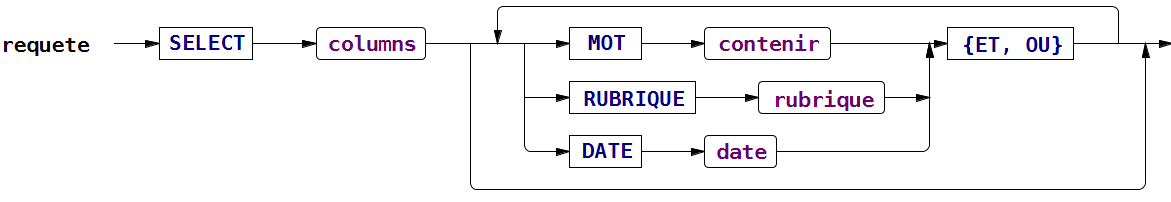
\includegraphics[width=1\textwidth]{images/grammaire.png}
    \caption{Génération d'arbre associé}
\end{figure}

\begin{figure}[H]
    \centering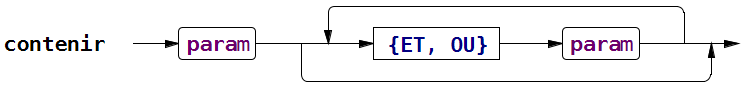
\includegraphics[width=1\textwidth]{images/param.png}
    \caption{Gestion de plusieurs paramètres avec conjectures}
\end{figure}

\begin{figure}[H]
    \centering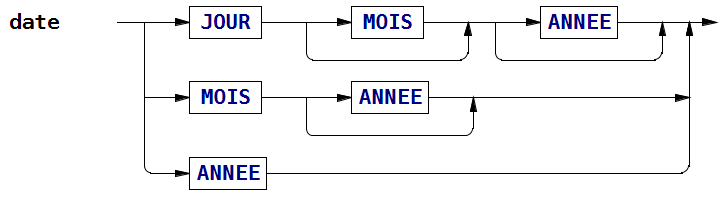
\includegraphics[width=1\textwidth]{images/date.png}
    \caption{Gestion des dates}
\end{figure}

\subsection{Règles}

Voici les règles que nous avons définies pour arriver à ce résultat :

\code{Règles}
\begin{lstlisting}
SELECT:'vouloir';

COLUMNS: 'fichier'|'numero'|'mot'|'email';

ET:'and';
OU:'or';

MOT:'contenir';

RUBRIQUE:'rubrique';

DATE:'date';
MOIS:('0'('1'..'9'))|'10'|'11'|'12';
ANNEE:('1'|'2')'0'..'9''0'..'9''0'..'9';
JOUR:('0'..'9')|(('1'|'2')'0'..'9')|'30'|'31';

WS:(' ' |'\t' | '\r' | 'je' | 'qui' | 'dont') {skip();} | '\n';

VAR:('A'..'Z' | 'a'..'z'|'\u00a0'..'\u00ff')(('a'..'z')|('0'..'9')|'-'|('\u00a0'..'\u00ff'))+;
\end{lstlisting}

À noter que l'ordre des tokens tel qu'il est donné dans la grammaire influe sur le parcours de l'arbre dans celle-ci et donc sur le traitement de la requête. Nous avons veillé à bien ordonner nos tokens.

\medskip

Ces règles sont assez explicites pour ne pas avoir besoin d'être expliquées, les explications fournies dans les sections précédentes étant suffisantes. On peut cependant préciser que \lstinline{WS} permet de ne pas tenir compte de certaines chaînes de caractères.

\section{Résultat actuel}

Exemple avec la phrase lemmatisée: \textit{vouloir fichier contenir voiture and rubrique focus and date 05 2011 and}.

\begin{figure}[H]
    \centering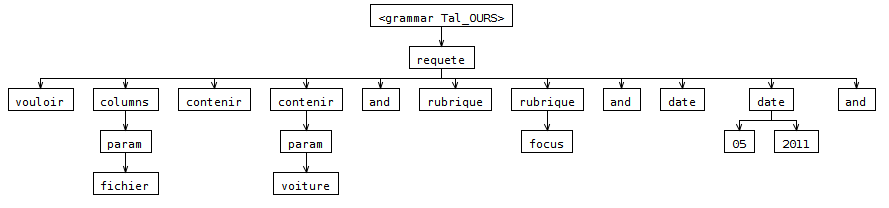
\includegraphics[width=1\textwidth]{images/arbre.png}
    \caption{Arbre généré}
\end{figure}

\noindent Ici, le ``and'' final sera retiré dans le post-traitement (qui est une méthode que l'on execute après avoir récupéré la requête SQL).

\bigskip
\bigskip

À l'heure actuelle, notre grammaire accepte des requêtes assez simples mais précises. Il conviendra d'ici à la fin du projet de considérer peut-être des recherches sur l'email, uniquement les titres, etc. Il faudra probablement étoffer notre post-traitement, qui est appliqué à la requête générée par Antlr, pour supporter également les \sql\lstinline{INNER JOIN}, nécessaires lors des recherches sur un texte contenant plusieurs mots.

\chapter{TD6: Interrogation d'une BDD SQL}

Dans le cadre de ce TD, une base de données PostgreSQL nous était accessible sur le réseau de l'UTC. Celle-ci est constituée de tables calquées sur les tables inverses réalisées durant les premiers TD portant sur ce projet. L'indexation ici était donc faite sur les fichiers en fonction des titres des articles, de leur date, leur rubrique, des numéros, emails, etc.

\section{Ambition}

Pour ce TD, il s'agissait de réaliser quelques tests d'interrogation de la base afin de se familiariser à la fois avec celle-ci mais aussi avec l'interrogation de bases en Java. Nous devions aussi vérifier si les résultats retournés étaient bien ceux attendus.

\medskip

Les requêtes SQL étaient dans un premier temps ``\textit{hardcodées}''. Nous avons ensuite dû permettre à l'utilisateur de rentrer sa requête à la main en la tapant.

\medskip

La légère difficulté résidait dans le traitement des résultats retournés. Dans l'hypothèse que n'importe quelle requête pouvait être tapée, on ne pouvait prédire à l'avance le nombre de colonnes dans les résultats.

\section{Programme générique acceptant n'importe quelle requête}
\java
Pour solutionner le problème susmentionné, il nous a fallu aller voir dans l'API SQL de Java les méthodes à notre disposition. Il se trouve qu'il existe un moyen d'obtenir les méta-données des résultats. En fonction de ces méta-données, nous étions en mesure de connaître le nombre de colonnes pour chaque résultat. En revanche, on ne pouvait pas connaître le type (\lstinline{int}, \lstinline{String}, etc.). Nous utilisons donc la classe générique \lstinline{Object} de Java avec sa méthode \lstinline{toString()} afin d'afficher le contenu d'une colonne pour un résultat.

\medskip

Nous avons créé une classe Java permettant de gérer l'ensemble des opérations sur la base de données.

\medskip

Notre méthode Java exécutant une requête donnée en paramètre retourne donc comme résultat\\
\lstinline{Tuple<ArrayList<String>,ArrayList<ArrayList<String>>>}, où \lstinline{Tuple} est une classe utilitaire que nous avons créée pour l'occasion, en plus de celle pour la base de données.

\java
\begin{lstlisting}
public static class Tuple<A,B> {
	public final A headers;
	public final B array;

	public Tuple(A a, B b) {
		this.headers = a;
		this.array = b;
	}
}
\end{lstlisting}

Dans le résultat retourné, le membre A de notre tuple contient les headers (donc les noms des colonnes, récupérés grâce aux méta-données). Quant au membre B, il contient l'ensemble des lignes de résultats, où une ligne est un ensemble de colonnes, d'où l'\lstinline{ArrayList} contenant un \lstinline{ArrayList}. Utiliser des \lstinline{ArrayList} et non des tableaux classiques \lstinline{String[]} nous permet d'être plus souple quant à la taille des tableaux, en déléguant ce problème à cette classe. En effet nous ne connaissons pas à l'avance les tailles de résultat.

\section{Interrogation de la base de données}

Notre classe \lstinline{Database} permet de se connecter à la base de données et d'exécuter des requêtes quelconques sur celle-ci grâce à ses méthodes \lstinline{getConnection} (la connection se fait à l'aide du login, du mot de passe et de l'URL) et \lstinline{doRequest}.
La requête SQL exécutée dans la méthode \lstinline{doRequest} parcourt les tables nécessaires de la BDD et retourne les résultats sous forme de tuple.

\medskip

Une fois cette petite application Java permettant d'interroger la base de données obtenue, l'intérêt était de la lier au reste des TD composant le projet.

\chapter{Mise en commun pour le projet}

Le but final de ces différents TD est de les rassembler pour obtenir une seule application Java permettant de taper au clavier en entrée une requête en langage naturel de type "Je veux tous les articles parlant de nanotechnologie" et d'obtenir les résultats de celle-ci les plus précis possibles en sortie.
Il est donc nécessaire de combiner en une seule interface :
\begin{itemize}
  \item la correction orthographique : tout d'abord 'tokenizer' notre phrase d'entrée à l'aide des lexiques de lemmes et des stop lists
  \item grammaire Antlr : transformer cette phrase simplifiée en une requête SQL et éventuellement la post-traiter pour en faire une requête SQL valide
  \item l'API Java pour PostgreSQL : cette interface Java/PostgreSQL doit enfin exécuter la requête SQL obtenue sur la base de données mise à disposition et retourner les résultats en sortie de manière exploitable pour éventuellement les afficher ensuite sur une page web
\end{itemize}

\java
Nous avons fait tout cela dans une class \lstinline{Main} qui contient la fonction \lstinline{main}. Cette fonction appelle des méthodes de l'ensemble des classes mentionnées plus haut afin d'appliquer les traitements dans le bon ordre, en commençant par demander une requête à l'utilisateur. Grâce à une boucle infinie s'arrêtant quand l'utilisateur entre une requête vide, nous sommes capables de ne pas interrompre le programme et de redemander autant de requêtes que l'utilisateur le souhaite.

\begin{figure}[H]
    \centering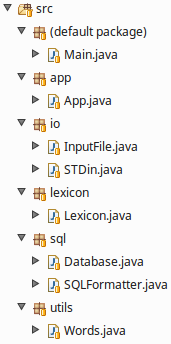
\includegraphics[width=0.25\textwidth]{images/projet.png}
    \caption{Ensemble du projet}
\end{figure}

Toutes les classes ont déjà été décrites dans ce rapport sauf trois :

\begin{itemize}
  \item \lstinline{App.java} : contient une constante utile à toutes les classes pour du debug, pour savoir quoi afficher dans la console :
      \java
        \begin{lstlisting}
public static final boolean DEBUG = true;
        \end{lstlisting}
  \item \lstinline{Words.java} : contient des méthodes \lstinline{static} pour nettoyer les différentes \lstinline{String} que nous manipulons (enlever les doubles espaces, faire des \lstinline{trim()}, etc.)
  \item \lstinline{SQLFormatter.java} : contient deux méthodes \lstinline{static}, nos pré et post-traitements
\end{itemize}

\medskip

Bien entendu, une fois toutes ces étapes réalisées, le travail de recherche n'est pas pour autant terminé car il peut être intéressant de prendre en compte les analyses sémantiques et pragmatiques par exemple, en plus de l'analyse syntaxique. Le nombre de requêtes en langage naturel possible étant potentiellement illimité, il est toujours possible de raffiner plus précisément le traitement de ces requêtes ; on peut par exemple avoir des requêtes portant sur plusieurs sujets différents, demandant des articles entre deux dates ou sur une période de temps, etc. Il sera intéressant d'essayer de perfectionner notre grammaire, le pré-traitement avec de donner la requête à la grammaire ainsi que le post-traitement, après avoir récupéré la sortie de la grammaire et avant d'exécuter la requête SQL.

\medskip

L'idée finale est d'obtenir une application parée à toute éventualité face à un utilisateur lambda qui est susceptible de demander n'importe quelle requête, portant sur n'importe quel sujet, à n'importe quelle date, etc.

\chapter{Conclusion}

À travers l'intégralité de ces différents TD, nous avons pu découvrir les méthodes liées à l'indexation et la recherche de l'information étape par étape. D'abord par la structuration d'information brut en un corpus XML puis la création de tables inverses de lemmes et d'une stop list ; ensuite par un travail de réflexion et d'analyse sur la correction orthographique d'une phrase entrée par un utilisateur ; et enfin par l'analyse lexicale et syntaxique d'une requête en langage naturel à l'aide d'une grammaire SQL.

\medskip

Ces différentes étapes furent ensuite amenées à être rassemblées en une seule application, qui sert d'interface entre l'utilisateur demandant une requête et la base de données questionnée.

\medskip

L'objectif idéal pour ce projet final serait d'obtenir une application à même de traiter presque n'importe quelle requête, quelle que soit la formulation de cette dernière ou le nombre de critères demandés, en prenant en considération les fautes de frappe (et pas seulement les inversions de lettres), etc.


%%%%%%%%% APPENDICES %%%%%%%%%
\begin{appendices}
\chapter{Correction orthographique}\label{corr}

\java
\begin{lstlisting}
/**
 * Essaye de détecter une inversion et corrige un score de Levenshtein
 * @param word Le mot pour lequel on cherche un lemme
 * @param comparedTo Le lemme potentiel
 * @param score Le score de Levenshtein obtenu pour ces deux mots
 * @return Le nouveau score pondéré
 */
private double testInversions(String word,String comparedTo, int score){
	double newScore = (double) score;
	switch (score) {
	case 0:
		return (double)0;
	default:
		break;
	}

	boolean problem = false;
	for (int i = 0; i < word.length() && i < comparedTo.length(); i++) {
		if (word.charAt(i) == comparedTo.charAt(i))
			continue;
		else if (!problem) {
			problem = true;
			if (i + 1 < comparedTo.length() && word.charAt(i) != comparedTo.charAt(i+1)) {
				break;
			}
		}
		else if (problem) {
			if (word.charAt(i) == comparedTo.charAt(i - 1)) {
				problem = false;
				// C'était une inversion
			}
			else {
				break;
			}
		}
	}
	newScore = !problem && word.length() == comparedTo.length() ?
			0
			:
			(word.length() == comparedTo.length() ?
						newScore - 0.1
						:
							newScore);

	return newScore;
}
\end{lstlisting}


\end{appendices}

\end{document}
